\documentclass[a4paper,12pt, dutch, oneside ]{book}

\usepackage[dutch]{babel}
\usepackage[utf8]{inputenc}
\usepackage{listings}

\usepackage{graphicx}
\graphicspath{ {./figuren/} }

\usepackage{Sweave}
\begin{document}


%\author{}
\title{R voor humane wetenschappen}
\date{September 2023}

%\maketitle
%\tableofcontents

%\chapter{Installatie}

%\include{"software"}

%\chapter{Werking}

%\section{Data}

\section{Bewerkingen}

\begin{Schunk}
\begin{Sinput}
> attach(mtcars)
> plot(wt, mpg)
> abline(lm(mpg~wt))
> title("Regressie van MPG en Weight")
> 
\end{Sinput}
\end{Schunk}
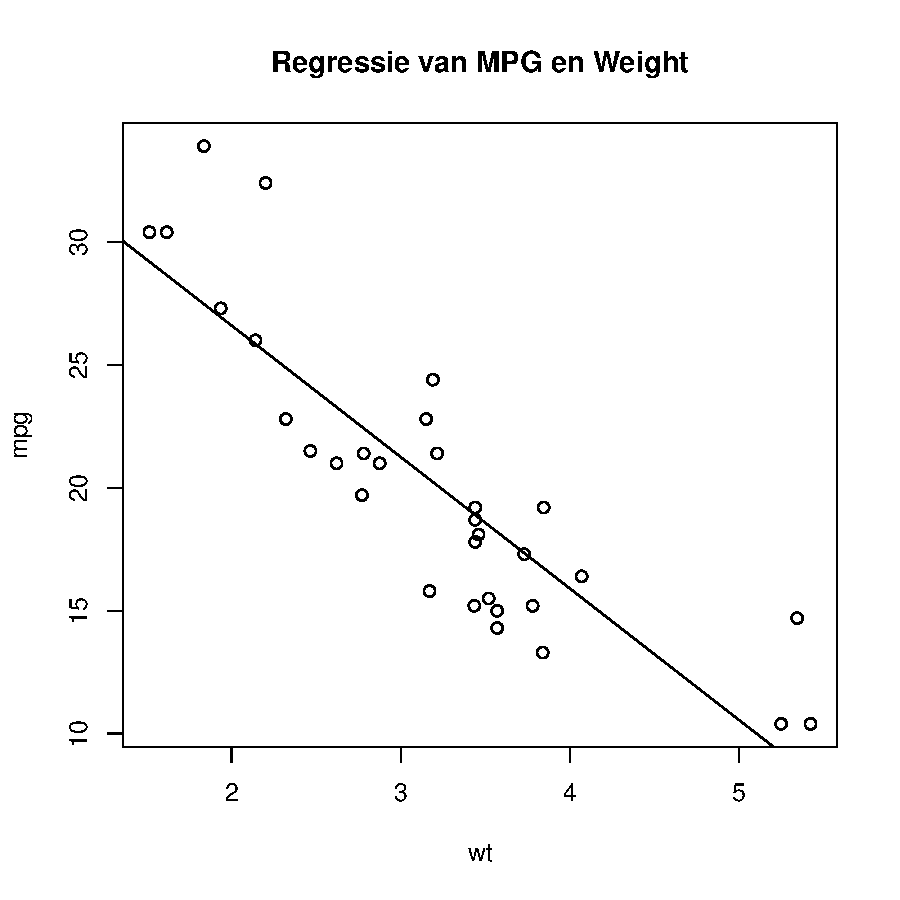
\includegraphics{hoofd-t}

% 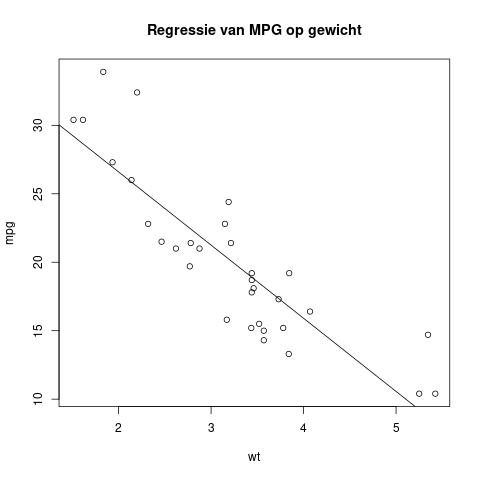
\includegraphics[scale=.5]{ren.jpeg}
% \begin{lstlisting}[language=R]
%     attach(mtcars)
%     plot(wt, mpg)
%     abline(lm(mpg~wt))
%     title("Regression van MPG op Weight")
% \end{lstlisting}

\section{Dynamische R code}
\begin{Schunk}
\begin{Sinput}
> # Create a sequence of numbers
> X = 2:10
> # Display basic statistical measures
> summary(X)
\end{Sinput}
\begin{Soutput}
   Min. 1st Qu.  Median    Mean 3rd Qu.    Max. 
      2       4       6       6       8      10 
\end{Soutput}
\begin{Sinput}
> 
\end{Sinput}
\end{Schunk}

\subsection{Histogrammen}
\begin{Schunk}
\begin{Sinput}
> # Inladen gegevens
> str(airquality)
\end{Sinput}
\begin{Soutput}
'data.frame':	153 obs. of  6 variables:
 $ Ozone  : int  41 36 12 18 NA 28 23 19 8 NA ...
 $ Solar.R: int  190 118 149 313 NA NA 299 99 19 194 ...
 $ Wind   : num  7.4 8 12.6 11.5 14.3 14.9 8.6 13.8 20.1 8.6 ...
 $ Temp   : int  67 72 74 62 56 66 65 59 61 69 ...
 $ Month  : int  5 5 5 5 5 5 5 5 5 5 ...
 $ Day    : int  1 2 3 4 5 6 7 8 9 10 ...
\end{Soutput}
\begin{Sinput}
> #Example 1: Simple histogram
> Temperature <- airquality$Temp
> hist(Temperature)
> # Example 2: Histogram with added parameters
> hist(Temperature,
+ main="Maximum daily temperature at La Guardia Airport",
+ xlab="Temperature in degrees Fahrenheit",
+ xlim=c(50,100),
+ col="darkmagenta",
+ freq=FALSE
+ )
> # Return Value of hist()
> h <- hist(Temperature)
> h
\end{Sinput}
\begin{Soutput}
$breaks
 [1]  55  60  65  70  75  80  85  90  95 100

$counts
[1]  8 10 15 19 33 34 20 12  2

$density
[1] 0.010457516 0.013071895 0.019607843 0.024836601 0.043137255 0.044444444
[7] 0.026143791 0.015686275 0.002614379

$mids
[1] 57.5 62.5 67.5 72.5 77.5 82.5 87.5 92.5 97.5

$xname
[1] "Temperature"

$equidist
[1] TRUE

attr(,"class")
[1] "histogram"
\end{Soutput}
\begin{Sinput}
> # Example 3: Use Histogram return values for labels using text()
> h <- hist(Temperature,ylim=c(0,40))
> text(h$mids,h$counts,labels=h$counts, adj=c(0.5, -0.5))
> # Example 4: Histogram with different breaks
> hist(Temperature, breaks=4, main="With breaks=4")
> hist(Temperature, breaks=20, main="With breaks=20")
> #Example 5: Histogram with non-uniform width
> hist(Temperature,
+ main="Maximum daily temperature at La Guardia Airport",
+ xlab="Temperature in degrees Fahrenheit",
+ xlim=c(50,100),
+ col="chocolate",
+ border="brown",
+ breaks=c(55,60,70,75,80,100)
+ )
> 
\end{Sinput}
\end{Schunk}


\chapter{Toepassingen}
wat moeten de leerlingen kunnen ?

\section{Voor het vak wiskunde}
De leerplandoelen van het onderdeel \textbf{Combinatieleer, kansrekenen, statistiek}

\begin{description}
\item[LPD27 SMD + GO!]De leerlingen lossen telproblemen op met en zonder herhaling en waarbij de volgorde al dan niet van belang is.
\begin{itemize}
    \item De leerlingen lossen telproblemen zonder herhaling op met combinaties. De leerlingen lossen telproblemen op met en zonder herhaling en waarbij de volgorde al dan niet van belang is.
    \item Standaard Combinatoriek
\end{itemize}

\item[LPD28 BV 06.13] De leerlingen bepalen kansen met behulp van kruistabellen, boomdiagrammen en de wet van Laplace.
\begin{itemize}
    \item Verband tussen relatieve frequentie en kans.
    \item Standaard Kansrekenen
\end{itemize}

\item[LPD29 GO!] De leerlingen bepalen het afhankelijk zijn van gebeurtenissen.
\begin{itemize}
    \item Voorwaardelijke kans
    \item  Standaard Voorwaardelijke kans + Kruistabellen
\end{itemize}

\item[LPD30 BV 06.14] De leerlingen verklaren het belang van randomisatie en representativiteit bij steekproeven voor het formuleren van statistische besluiten over een populatie.
\begin{itemize}
    \item Variabiliteit van steekproeven. Aselecte steekproef.
    \item Cursus Callaert steekproefmethoden.
    \item Link met Humane vakken.
    \item Link met Economie?
\end{itemize}

\item[LPD31 GO!] De leerlingen analyseren het verband tussen twee numerieke grootheden in een dataset met behulp van een spreidingsdiagram.
\begin{itemize}
    \item Trendlijn. Lineaire regressie. Correlatiecoëfficiënt.
    \item Cursus Callaert, aangevuld met lesnota's.
\end{itemize}

\item[LPD31 BV 06.15] De leerlingen leggen in concrete situaties het verschil uit tussen samenhang en causaliteit.
\begin{itemize}
    \item Verwachtingswaarde, standaardafwijking.
    \item Link met Humane vakken.
    \item Link met Economie?
\end{itemize}

\item[LPD32 SMD] De leerlingen berekenen en interpreteren kansen met behulp van de binomiale verdeling
\begin{itemize}
    \item Standaard Binomiale
\end{itemize}

\item[LPD33 BV 06.16] De leerlingen gebruiken de normale verdeling als continu model bij gegeven data.
\begin{itemize}
    \item Grafische beoordeling van de toepasbaarheid van het model. Rekenkundig gemiddelde en de standaardafwijking van de gegeven data als schatting voor de parameters van het model. Grafische betekenis van gemiddelde en standaardafwijking van een normaal verdeelde kansvariabele in termen van de Gausskromme.
    \item Standaard Normale aangevuld met lesnota's over grafische beoordeling (naast histogram ook q-q-plot)
\end{itemize}

\item[LPD34 BV 06.17] De leerlingen berekenen kansen bij een normaal verdeelde kansvariabele.
\begin{itemize}
    \item Standaard Normale
\end{itemize}

\item[LPD35 SMD] De leerlingen leggen in betekenisvolle situaties de betekenis van betrouwbaarheidsniveau, betrouwbaarheidsinterval en foutenmarge uit.
\begin{itemize}
    \item Steekproefverdeling (gemiddelde en standaardafwijking). Verband met steekproefgrootte en standaardafwijking.
    \item Cursus Callaert aangevuld met lesnota's over de wortel-n-wet
\end{itemize}

\item[LPD36 SMD] De leerlingen toetsen hypothesen.
\begin{itemize}
    \item Nulhypothese, alternatieve hypothese, p-waarde, significantieniveau
    \item Cursus Callaert aangevuld met lesnota's over de wortel-n-wet
    \item Link met Humane vakken.
    \item Link met Economie?
\end{itemize}

\item[LPD37 SMD] De leerlingen analyseren grote datasets met behulp van statistische software in functie van een statistisch onderzoek.
\begin{itemize}
    \item Deze cursus met R.
    \item Link met Humane vakken.
    \item Link met Economie
\end{itemize}
\end{description}

\section{Voor OC}
\end{document}
